\subsection{JDBC工作原理概述}
\begin{frame}[allowframebreaks,fragile]{JDBC工作原理概述}
\begin{itemize}
    \item JDBC (\textbf{J}ava \textbf{D}ata\textbf{B}ase \textbf{C}onnection)
    \begin{itemize}
        \item 由于不同的数据库管理系统的存在,在某个关系数据库管理系统下编写的应用程序就不能在另一个关系数据库管理系统下运行  
        \item 许多应用程序需要共享多个部门的数据资源,访问不同的关系数据库管理系统
    \end{itemize}
    \item JDBC 是面向Java 语言的软件开发工具包(Java Development Kit,JDK)中有关数据库的一个组成部分, 其提供了一组访问数据库的应用程序编程接口(Application Programming Interface,API)
    \item JDBC约束力
    \begin{itemize}
        \item 规范应用开发
        \item 规范关系数据库管理系统应用接口
    \end{itemize}
    \framebreak
    \begin{itemize}
        \item JDBC应用系统的体系结构 
        \begin{enumerate}
            \item 用户应用程序 
            \item JDBC驱动程序管理器 
            \item 数据源
        \end{enumerate}
    \end{itemize}
    \framebreak
    \begin{figure}
        \centering
        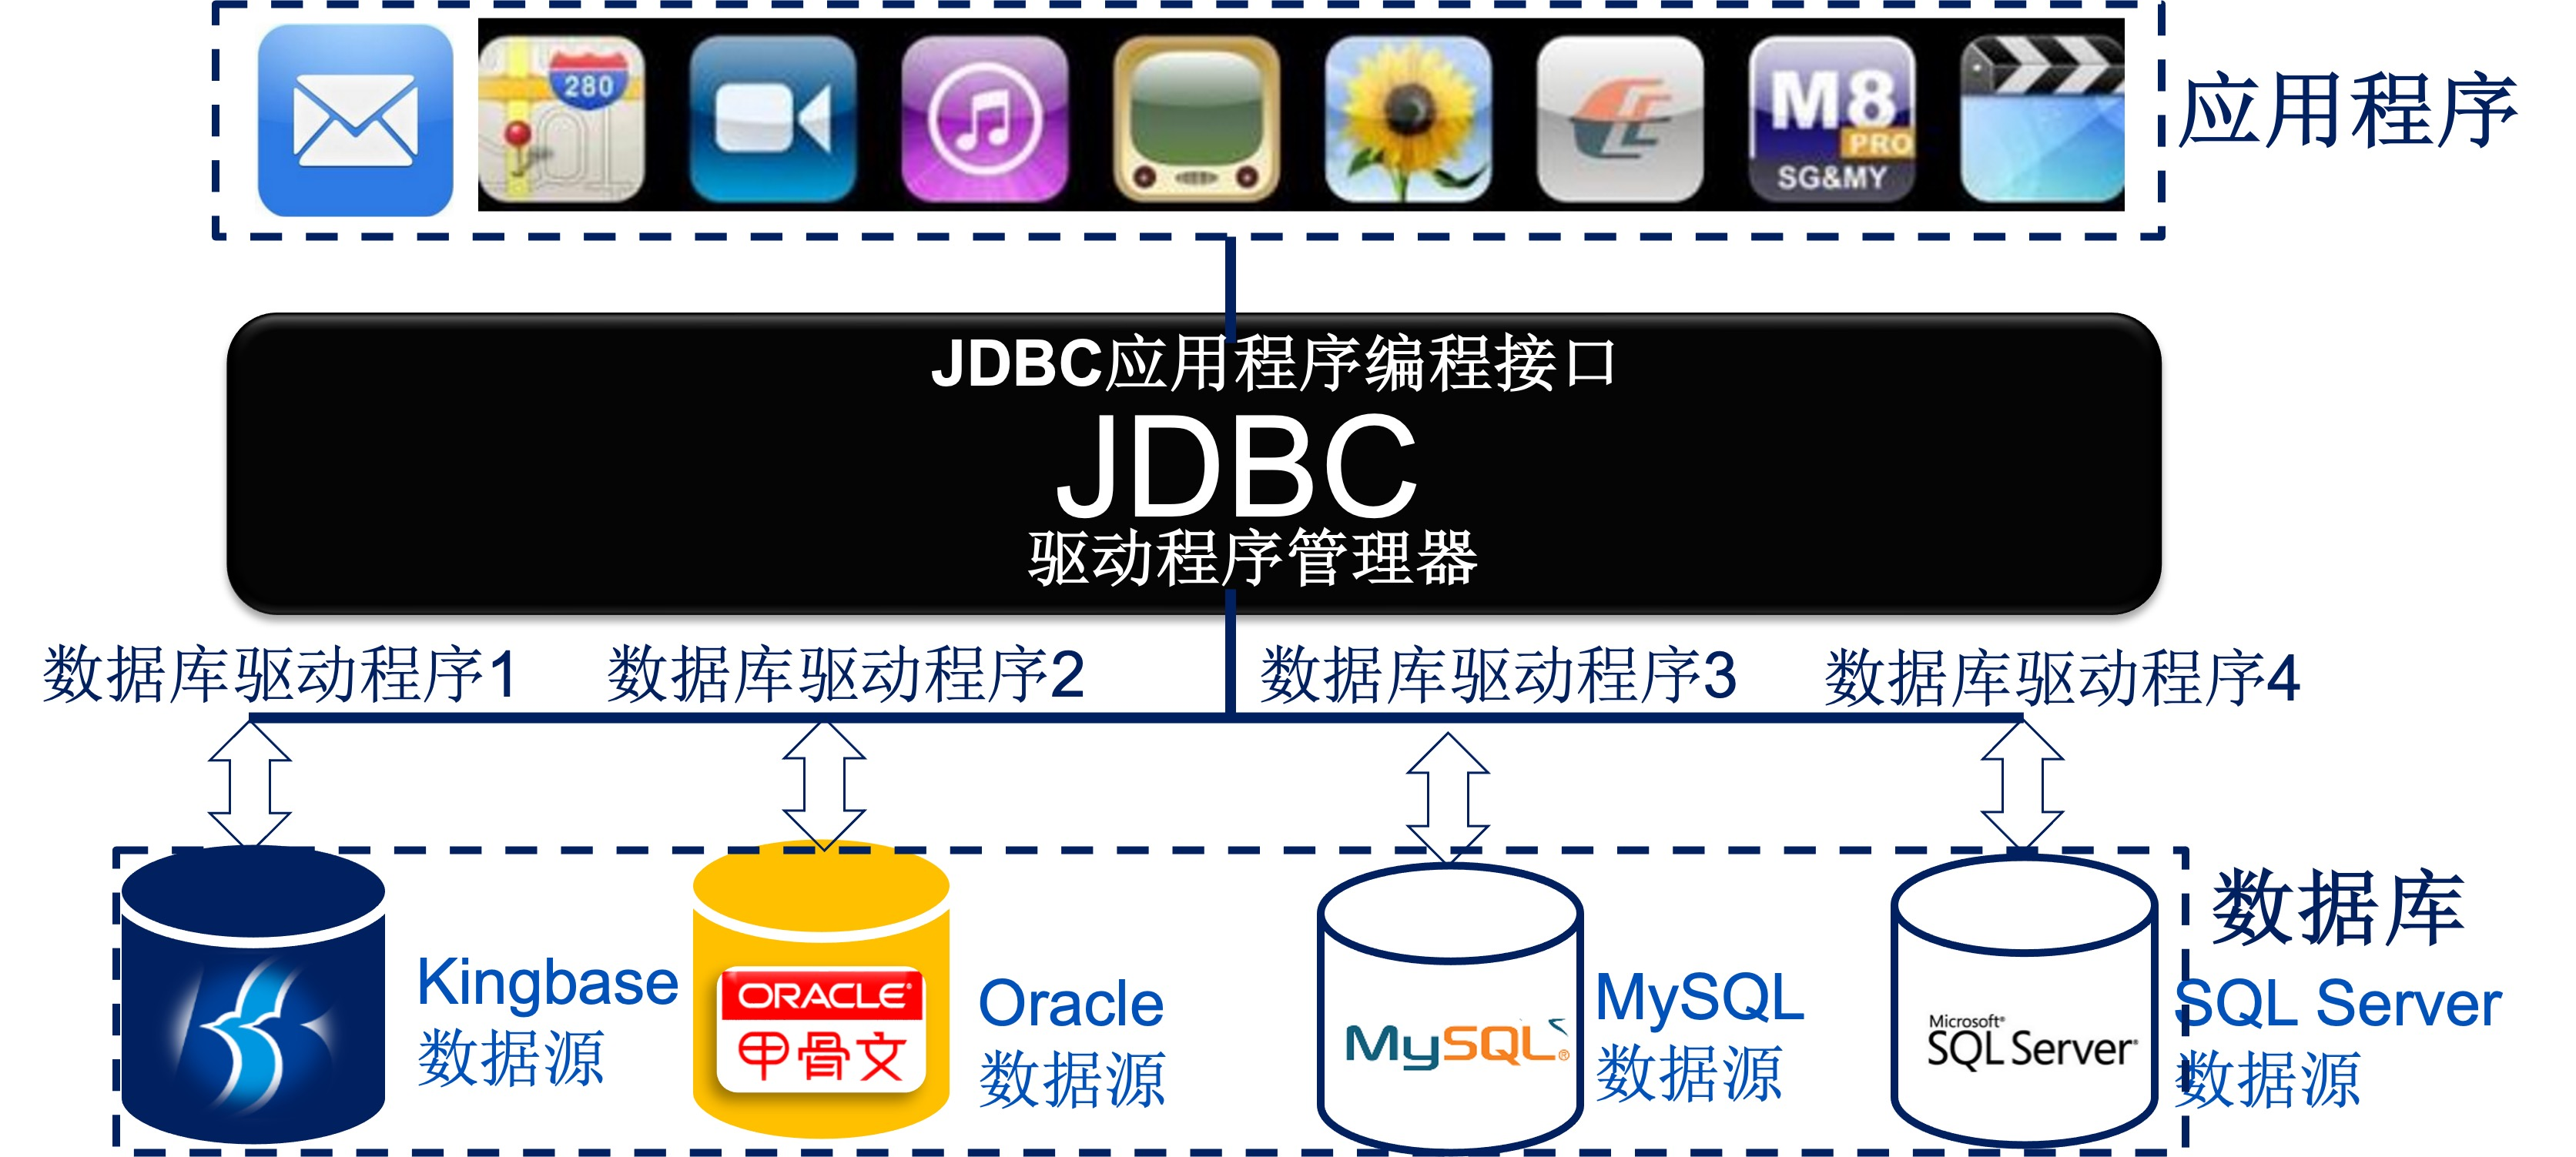
\includegraphics[width=0.9\textwidth]{figure/fig-10.jpg}
    \end{figure}
\end{itemize}
\end{frame}


\subsection{JDBC APIs基础}
\begin{frame}[allowframebreaks,fragile]{JDBC APIs基础}
\begin{itemize}
    \item JDBC中的常用类
    \begin{itemize}
        \item JDBC进行应用程序开发涉及到的所有类都包含在java.sql包中
        \item 不同的JDBC版本接口名和使用略有差异
    \end{itemize}
    \begin{figure}
        \centering
        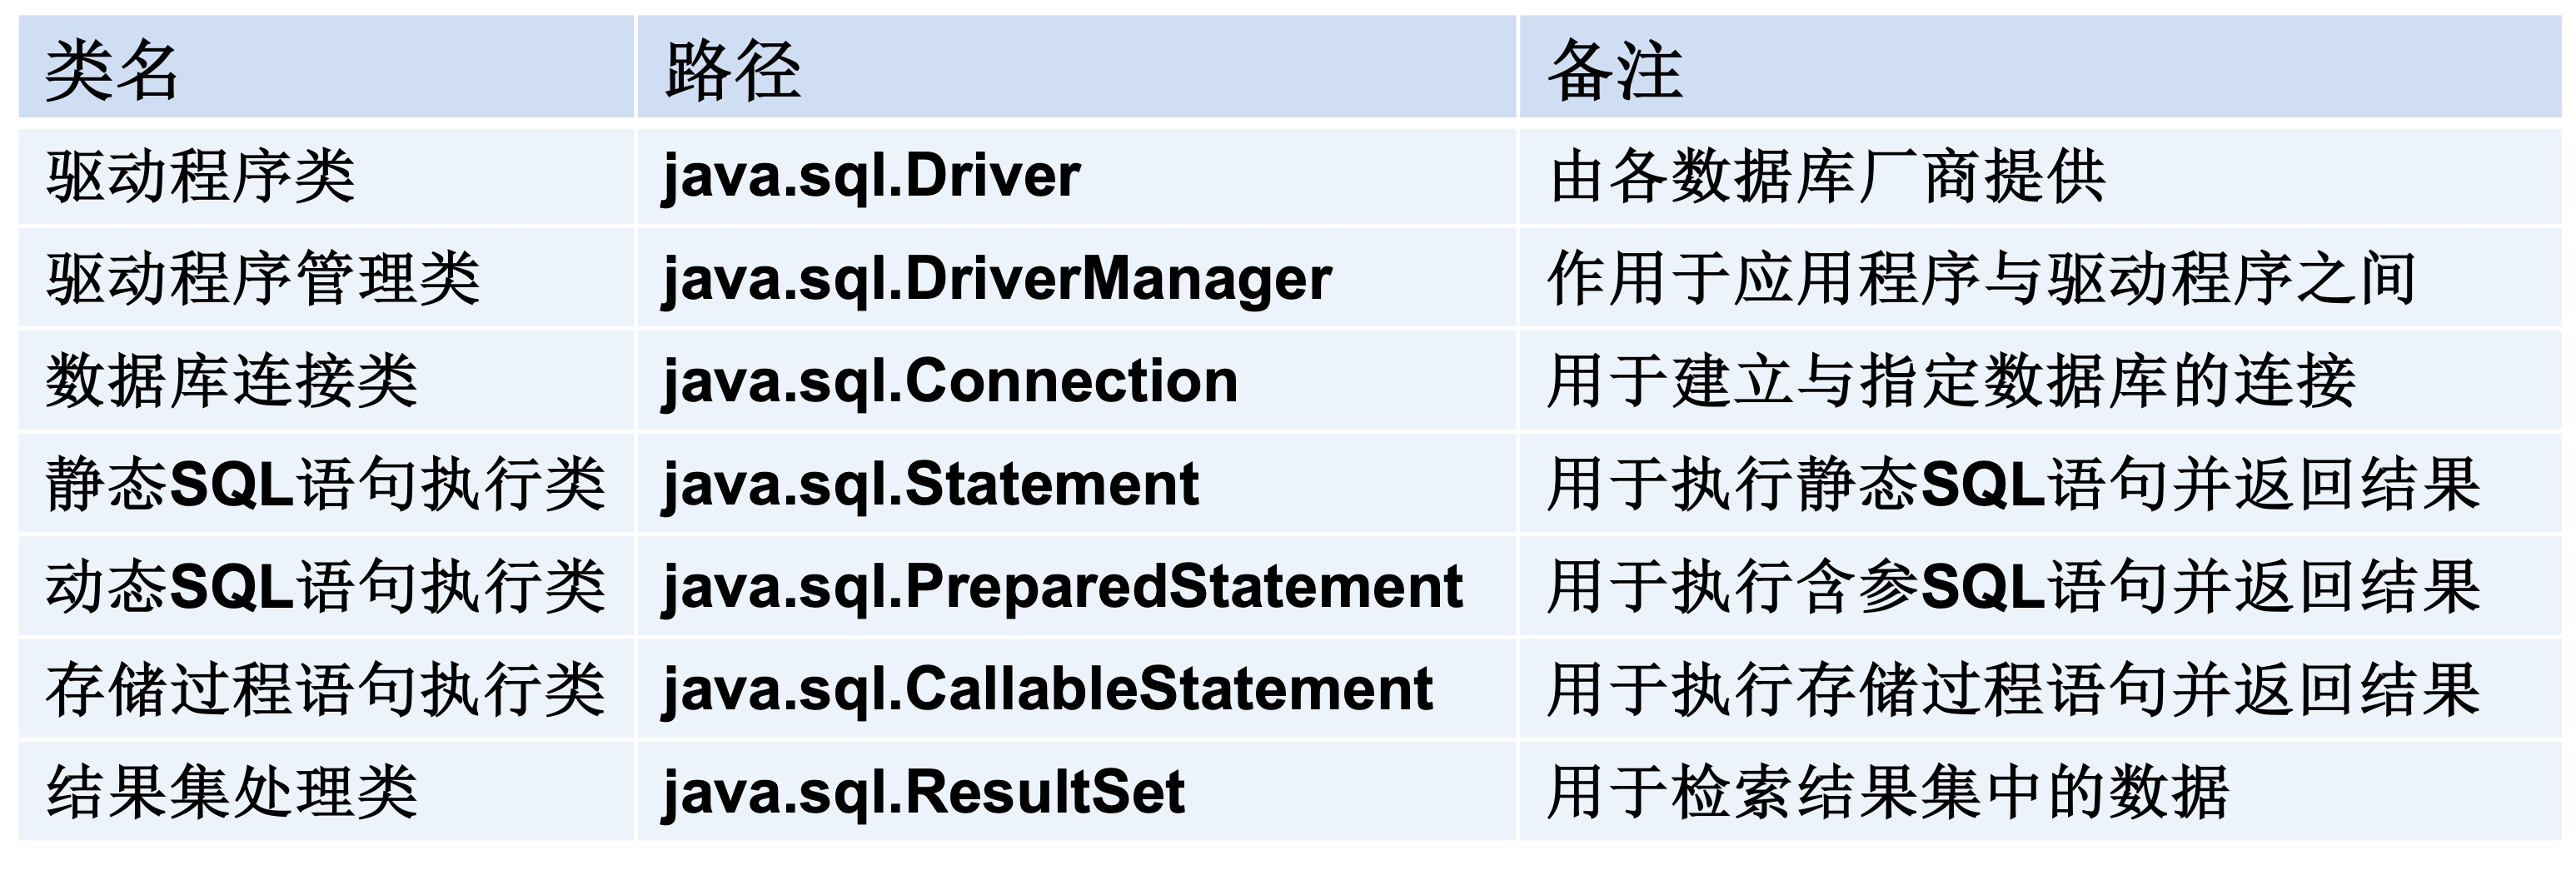
\includegraphics[width=0.9\textwidth]{figure/fig-11.jpg}
    \end{figure}
    \framebreak
    \item 数据类型
    \item 由数据库管理系统的驱动程序完成自身数据类型和JDBC标准数据类型的映射
    \begin{itemize}
        \item SQL数据类型:用于数据源
        \begin{itemize}
            \item VARCHAR、 CHAR 、 BIT 、NUMERIC、DATE等
        \end{itemize}
        \item Java数据类型:用于应用程序的Java代码
        \begin{itemize}
            \item String、boolean、BigDecimal、byte、short、int等
        \end{itemize}
    \end{itemize}
    
\end{itemize}
    \begin{table}[!htp]
        \centering
        \resizebox{0.7\textwidth}{!}{
        \begin{tabular}{c|c|c}
        \toprule
             & SQL数据类型 & Java数据类型 \\
        \midrule
             SQL数据类型 & 数据源之间转换 & 应用程序变量传递给语句 \\
            Java数据类型 & 从数据库中读取数据赋值给应用程序变量 & 应用程序变量之间转换\\
        \bottomrule
        \end{tabular}
        }
        \caption{SQL数据类型和java数据类型之间的转换规则}
        \label{tab:my_label}
    \end{table}
\end{frame}
\subsection{使用JDBC操纵数据库的工作流程}
\begin{frame}[allowframebreaks,fragile]{使用JDBC操纵数据库的工作流程}
\begin{enumerate}
    \item 步骤1:加载驱动程序
    \item 步骤2:建立与数据库的连接
    \begin{itemize}
        \item 定义连接的URL
        \item 利用生成的URL建立与数据库的连接
    \end{itemize}
    \item 步骤3:执行SQL语句
    \begin{itemize}
        \item 创建语句执行类对象
        \item 执行SQL语句,可以通过executeQuery、 executeUpdate、 execute三种方式执行
    \end{itemize}
    \item 步骤4:处理结果集
    \item 步骤5:释放资源
\end{enumerate}
\end{frame}


\begin{frame}[allowframebreaks,fragile]{使用JDBC操纵数据库的工作流程}
\begin{enumerate}
    \item 步骤1:加载驱动程序
    \begin{itemize}
        \item 驱动程序在JDBC API中实现定义数据交互的接口
        \item  【例8.7】对Kingbase、Oracle、SQL Server加载数据库驱动
\begin{block}{}
\begin{lstlisting}[language=Java, linewidth=\textwidth]
Class.forName("com.kingbase.Driver");       /* Kingbase */
Class.forName("oracle.jdbc.OracleDriver");  /* Oracle */
Class.forName(“com.microsoft.jdbc.sqlserver.SQLServerDriver”;   
/* SQL Server */
\end{lstlisting}
\end{block}
    \end{itemize}
\framebreak
    \item 步骤2:建立与数据库的连接
\begin{itemize}
    \item 加载驱动后,可以通过URL地址与数据库建立连接
    \item URL包含了连接数据库所需的协议、子协议和数据库名称,定义格式为:
    
    <协议名>:<子协议名>:<数据库名称>
    \item 【例8.8】定义与Kingbase、Oracle、SQL Server数据库连接的URL
\begin{block}{}
\begin{lstlisting}[language=Java, linewidth=\textwidth]
strURL = "jdbc:kingbase://" + 服务器名 +  ":" + 端口号 + "/" + 数据库名;
strURL = "jdbc:oracle:thin:@" + 服务器名 + ":" + 端口号 + ":" + 数据库名
strURL = "jdbc:microsoft:sqlserver://" + 服务器名 + ":" + 端口号 + ":" + 数据库名
// Kingbase、Oracle、SQL Server的默认端口号分别为54321、1521、1433
\end{lstlisting}
\end{block}
    \framebreak
    \item 【例8.9】建立与Kingbase数据库的连接,假定服务器地址为192.168.0.118,端口为54321,数据库名为DB-Student,用户名为Info001,密码为123456
    
\begin{block}{}
\begin{lstlisting}[language=Java, linewidth=\textwidth]
String strURL ="jdbc:kingbase:// 192.168.0.118:54321/DB-Student";
Connection conn= DriverManager.getConnection(strURL," Info001","123456");
\end{lstlisting}
\end{block}
\end{itemize}
    \framebreak
    \item 步骤3:执行SQL语句
    \begin{itemize}
        \item 静态语句执行类对象(Statement)
        \item 派生执行类对象:
            \begin{itemize}
                \item 动态语句执行类(PreparedStatement):执行动态的SQL语句
                \item 存储过程执行类(CallableStatement):执行数据库存储过程
            \end{itemize}
        \item 执行方法
            \begin{itemize}
                \item ResultSet executeQuery(): 执行数据库查询语句
                \item int executeUpdate(): 处理增、删、改以及定义语句
                \item boolean execute(): 处理存储过程或动态SQL语句
            \end{itemize}
        \item SQL注入防御
        \begin{itemize}
            \item 预编译
            \item 正则过滤,输入验证,框架......
        \end{itemize}
    \framebreak
        \item 【8.10】使用JDBC向课堂评价表中插入一条记录
\begin{block}{}
\begin{lstlisting}[language=Java, linewidth=\textwidth]
PreparedStatement stmt = conn.prepareStatement("INSERT INTO SC VALUES(?,?,?,?,?,?)");
/* 生成PreparedStatement类对象中的动态参数,注意第六个字段Feedback,未设置输入值 */
stmt.setString(1, " 20180001 ");    /*设置学生学号*/
stmt.setString(2, "19950018");  /*设置职工号*/
stmt.setString(3, "81001-01");  /*设置教学班号*/
stmt.setString(4, “老师讲得很出色");   /*设置学生评价意见*/
stmt.setBoolean(5,true);    /*设置学生评价意见类型*/
stmt.executeUpdate();
\end{lstlisting}
\end{block}    \end{itemize}


    \framebreak
    \item 步骤4:处理结果集
    \begin{itemize}
        \item ResultSet: 结果集合类对象
        \begin{itemize}
            \item .GetXXX(参数): 
        
            获取元组的属性值,XXX代表某种数据类型
            
            可以指定参数为列号(JDBC的列从1开始)或列名
            
            \item 游标(cursor):JDBC处理结果集的机制

            TYPE\_FORWARD\_ONLY:只能向下滚动(默认类型)
            
            TYPE\_SCROLL\_IN(SEN)SENSITIVE 双向滚动,区别为是否同步数据库更新操作
        \end{itemize}
    \framebreak
    \item 【8.12】遍历教师职工号为19950018,教学班号为81001-01的学生课程评价详情
\begin{block}{}
\begin{lstlisting}[language=Java, linewidth=\textwidth]
String SQL = "SELECT Sno, Assess, CAtype, Feedback FROM ClassAssess
  WHERE Tno='19950018' AND TCo = '81001-01'";
ResultSet rs = stmt.executeQuery(SQL);
while(rs.next()){
    String Sno = rs.getString("Sno");       /*等价于rs.getString(1)*/
    String strAssess = rs.getString("Assess");      /*等价于rs.getString(2) */
    Boolean bCAtype = rs.getBoolean ("CAtype");      /*等价rs.getBoolean (3) */
    String strFeedback = rs.getString("Feedback");  /*等价于rs.getString(4) */
    System.out.printf("[%s,%b,%s]%n", strAssess, bCAtype, strFeedback);
}
\end{lstlisting}
\end{block}


    \end{itemize}
  \framebreak
    \item 步骤5:释放资源
    \begin{itemize}
        \item 执行结束后,将与数据库进行交互的对象释放
        \item 释放资源有标准的顺序:
        \begin{itemize}
            \item 关闭结果集:ResultSet.close()
            \item 关闭语句执行类对象:Statement.close()
            \item 释放数据库连接对象:Connection.close()
        \end{itemize}
        \item 释放资源的Coding Tips
        \begin{itemize}
            \item Connection对象在应用程序中较为稀有,尽量做到晚创建,早释放
            \item 推荐在finally代码块中释放资源,以满足异常处理机制(finally语句在什么情况下都会执行,确保一定会释放资源)
        \end{itemize}
    \end{itemize}
\end{enumerate}
\end{frame}

\begin{frame}[allowframebreaks,fragile]{【例8.13】基于JDBC实现【任务4】}
\begin{columns}
\begin{column}{0.6\textwidth}
\vspace{-2ex}
\begin{itemize}
    \item 选课关系模式:
    \begin{itemize}
        \item SC(Sno,TCno, Grade)
    \end{itemize}
    \vspace{-1ex}
    \item 教师关系模式:
    \begin{itemize}
        \item Teacher(Tno, Tname, Ttitle, Tbirthdate, Dno)
    \end{itemize} 
    \vspace{-1ex}
    \item 教学班关系模式: 
    \begin{itemize}
        \item TeachingClass(TCno, Capacity, Semester, Cno)
    \end{itemize}
    \vspace{-1ex}
    \item 讲授关系模式:
    \begin{itemize}
        \item Teaching(TCno, Tno, isLeading) 
    \end{itemize}
    \vspace{-1ex}
    \item 课堂评价关系模式: 
    \begin{itemize}
        \item ClassAssess(Sno, Tno, TCno, Assess, CAtype, CRfeedback)
    \end{itemize}
\end{itemize}
\end{column}

\begin{column}{0.4\textwidth}
\begin{figure}
    \centering
    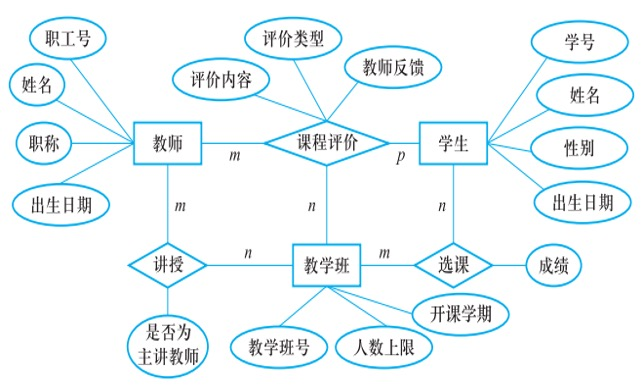
\includegraphics[width=\textwidth]{figure/fig-14.jpg}
\end{figure}
\end{column}

\end{columns}
\end{frame}


\begin{frame}[allowframebreaks,fragile]{【例8.13】基于JDBC实现【任务4】}
\begin{columns}
\begin{column}{0.4\textwidth}
\vspace{-2ex}
\begin{itemize}
    \item 数据库连接的管理
    \begin{itemize}
        \item 设置连接数据库的URL
        \item 创建连接数据库的静态函数
        \item 创建释放数据库连接对象的静态函数
    \end{itemize}
    \item 封装(步骤1-步骤2-步骤6)到数据库连接管理类中
\end{itemize}
\end{column}

\begin{column}{0.6\textwidth}
\vspace{-4ex}
\begin{block}{}
\begin{lstlisting}[language=Java, linewidth=\textwidth, basicstyle=\ttfamily\tiny]
public class ConnectionManager{
    static final String jdbcUrl="jdbc:kingdb://192.168.0.118:54321/DB-Student";
    static final String jdbcUsername = "Info001";
    static final String jdbcPassword = " 123456";
    private static Connection connection = null;
    /* 静态代码段, 加载Kingbase数据库驱动程序 */
    static {
        Class.forName("com.kingbase.Driver");
    }
    public static Connnection createConnection(){
        connection = DriverManager.getConnection(jdbcUrl, jdbcUsername, jdbcPassword);
        System.out.println("数据库连接成功");
        return connection;
    }
    /* 释放资源 */
    public static void release(){
        if (connection != null) connection.close();
        System.out.println("释放资源成功");
    }

}
\end{lstlisting}
\end{block}
\end{column}

\end{columns}
\end{frame}


\begin{frame}[allowframebreaks,fragile]{【例8.13】基于JDBC实现【任务4】}
\begin{columns}
\begin{column}{0.4\textwidth}
\vspace{-2ex}
\begin{itemize}
    \item 学生浏览指定的教学班和授课教师,并输入课程评价
    \item 完成步骤3-4
    \item 步骤3:创建语句对象
    \item 步骤4:执行语句对象
\end{itemize}
\end{column}

\begin{column}{0.6\textwidth}
\vspace{-4ex}
\begin{block}{}
\begin{lstlisting}[language=Java, linewidth=\textwidth, basicstyle=\ttfamily\tiny]
Connection conn = ConnectionManager.createConnection();
Statement stmnt = conn.createStatement();
/* 设置如下任务的SQL语句;获取学生所选的教学班及授课老师 */
/* 假设strSno为学生学号 */
String SQL4ClassAssess = "SELECT TCno, Tno FROM Student, Teacher, Teaching, SC WHERE Teacher.Tno=Teaching.Tno AND Teaching.TCno=SC.TCno AND SC.sno="+strSno;                          
\end{lstlisting}
\end{block}
\end{column}

\end{columns}
\end{frame}


\begin{frame}[allowframebreaks,fragile]{【例8.13】基于JDBC实现【任务4】}
\begin{columns}
\begin{column}{0.4\textwidth}
\vspace{-2ex}
\begin{itemize}
    \item 执行步骤5
    \begin{itemize}
        \item 根据结果集,执行用户的逻辑
        \item 构建学生课程评价的动态SQL语句
        \item 遍历学生选课的每一条记录,在动态SQL语句中设置学生对该门课程的评价,并更新该条记录
    \end{itemize}
    \item 执行步骤6
    \begin{itemize}
        \item 释放结果集、语句、连接对象
    \end{itemize}
\end{itemize}
\end{column}

\begin{column}{0.6\textwidth}
\vspace{-4ex}
\begin{block}{}
\begin{lstlisting}[language=Java, linewidth=\textwidth, basicstyle=\ttfamily\tiny]
ResultSet rs=stmnt.executeQuery(SQL4ClassAssess);
/* 设置插入学生课程评价的动态SQL语句 */
String insertSQL = "INSERT INTO ClassAssess(Sno, Tno, TCno, Assess, CAtype) VALUES(?,?,?,?,?)";
PreparedStatement ps = conn.prepareStatement(insertSQL);
while(rs.next){
    /* 阅读该学生所选的教学班及授课老师 */
    String strTno = rs.getString("Tno");
    String strTCno = rs.getString("TeachingClassNo");
    /* 对该授课教师讲授的教学班进行评价 */
    ps.setString(1, strSno);
    ps.setString(2, strTno);
    ps.setString(3, strTeachingClassNo);
    ps.setString(4, "老师讲得很好");
    /* 课程评价根据用户输入 */
    ps.setBoolean(5, true);
    ps.executeUpdate();
}
rs.close();
ps.close();
stmnt.close();
ConnectionManager.release();
\end{lstlisting}
\end{block}
\end{column}

\end{columns}
\end{frame}
